\section{三矩阵融合乘法算子设计}

\subsection{问题定义与目标分析}

传统实现通常将 $\mathbf{X}\mathbf{A}$ 的中间结果写回全局内存，再读取后继续计算 $\mathbf{T}\mathbf{B}$。本模板在这里保留少量示例文字，用于展示方案设计章节的写法和公式后的正文组织方式。

\subsection{整体设计框架}

图\ref{fig:trimm_framework} 给出了示例性的三矩阵融合框架图。模板中保留一张图片，便于检查图标题、交叉引用和图文间距是否满足排版预期。

\begin{figure}[htbp]
    \centering
    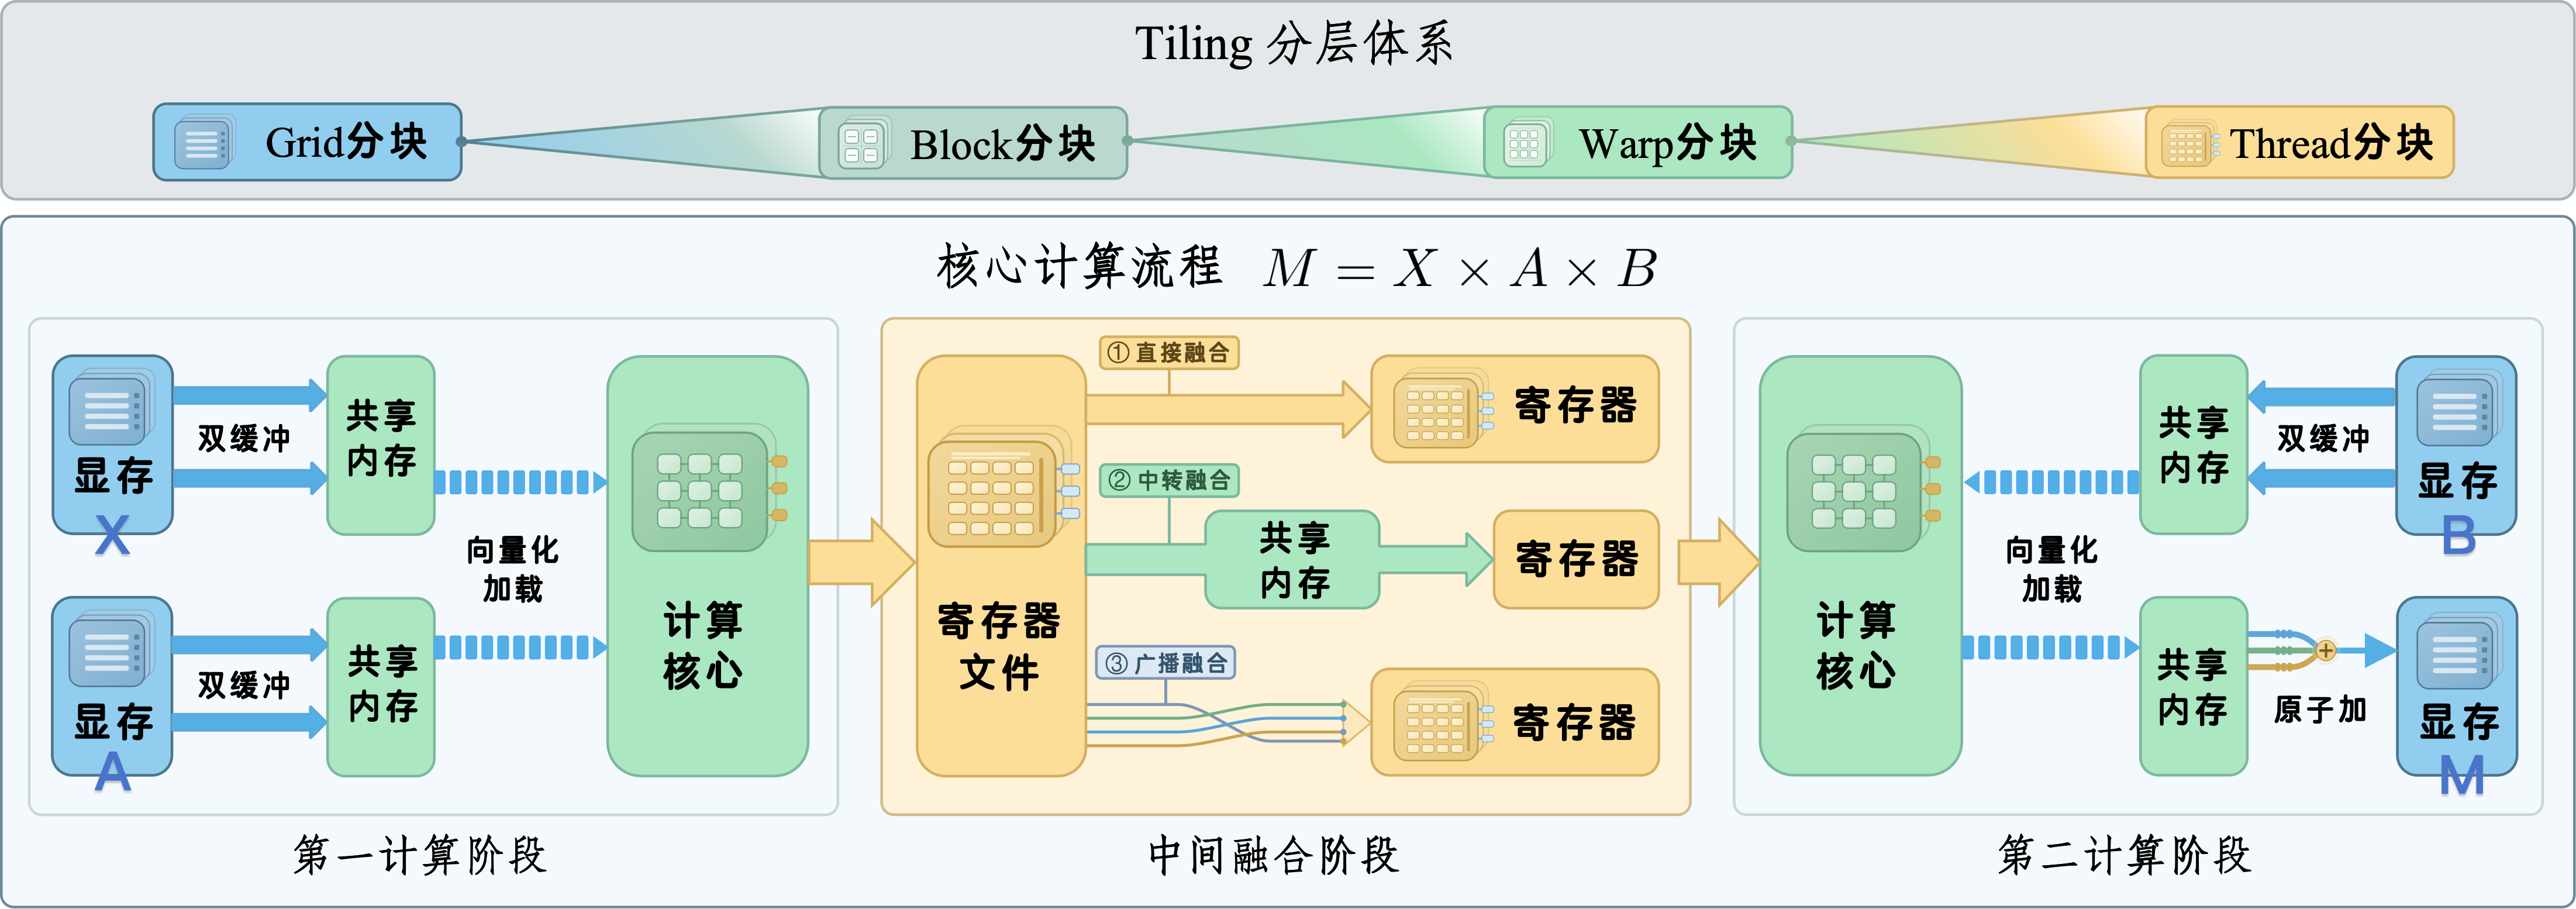
\includegraphics[width=\textwidth]{figures/trimm_framework.png}
    \caption{三矩阵融合算子的整体设计框架示例}
    \label{fig:trimm_framework}
\end{figure}

\subsection{融合思路示例}

示例主题中可以将融合策略简化为三类：寄存器转发、共享内存中转和面向 Tensor Core 的片段复用。这里不展开完整推导，只用少量内容占位，提醒使用者后续可按自己的论文需求继续细化。
